\documentclass[dvipdfmx]{beamer}

% packages
\usepackage[orientation=portrait,size=a0,scale=1.4]{beamerposter}
\usepackage[deluxe]{otf}
\usepackage{pxjahyper}
\usepackage{hyperref}
\usepackage{graphicx}
\usepackage{booktabs}
\usepackage{amsmath,amssymb}
\usepackage{bm}
\usepackage{ascmac}

\graphicspath{{../figures/}}
\makeatletter
\def\input@path{{../tables/}}
\makeatother

\renewcommand{\kanjifamilydefault}{\gtdefault}

\uselanguage{japanese}
\languagepath{japanese}
\deftranslation[to=japanese]{Figure}{図}
\deftranslation[to=japanese]{Table}{表}
\deftranslation[to=japanese]{References}{参考文献}

% theme
\usetheme{MyPoster}
\usefonttheme{professionalfonts}

% template
\setbeamertemplate{bibliography item}[text]
\setbeamertemplate{bibliography entry title}{}
\setbeamertemplate{bibliography entry location}{}
\setbeamertemplate{bibliography entry note}{}

\DeclareMathOperator{\MSE}{MSE}
\DeclareMathOperator{\var}{var}
\DeclareMathOperator{\cov}{cov}
\bmdefine{\x}{x}
\newcommand{\varm}{\var(\varepsilon_\theta|\x)}
\newcommand{\varh}{\var(\varepsilon_h)}
\newcommand{\covh}{\cov(\varepsilon_h)}
\newcommand{\covmh}{\cov(\varepsilon_\theta, \varepsilon_h)}

% title
\title{経済予測に関する人間と機械のアンサンブル法の考案}
\author{三吉 貴大, 松原 繁夫, 山本 章平, 辻 一真, 水嶋 舜人}
\institute{情報学研究科 社会情報学専攻 石田・松原研究室}
\date{2017年2月23日}

\begin{document}
\begin{frame}{}
  %%%%%%%%%%%%%%%%%%%%%%%%%%%%%%%%%%%%%%%%%%%%%%%%%%%%%%%%%%%%%%%%
  \begin{block}{はじめに: 研究の背景とアプローチ}
    \begin{columns}
      \begin{column}{.59\textwidth}
        \structure{背景: 経済予測}
        \begin{itemize}
          \item GDPやインフレなどの経済指標は,政策立案者や企業,投資家にとって重要
          \item マクロ経済モデルや時系列解析等の手法では,1,2年程度の短期の予測は困難
          \item 近年,集合知と機械学習による予測がそれぞれ注目されている
        \end{itemize}
        \smallskip
        \begin{columns}
          \begin{column}{.49\textwidth}
            \begin{itembox}[l]{\structure{人の集合知による予測}}
              \begin{itemize}
                \item 例: 質問紙調査の集計値
                \item 景気や政策などの情報を総合的に考慮して予測を行う
                \item 多様性を大きくすることで誤差の期待値を小さくできる
                % ~\cite{Page2008}
              \end{itemize}
            \end{itembox}
          \end{column}
          \begin{column}{.49\textwidth}
            \begin{itembox}[l]{\structure{機械学習による予測}}
              \begin{itemize}
                \item 例: 再帰型ニューラルネット
                \item 過去の時系列から統計的に予測器を構築し予測を行う
                \item 過去のデータを元に誤差の期待値を定量化できる
              \end{itemize}
            \end{itembox}
          \end{column}
        \end{columns}
        \smallskip
        \begin{center}
          \alert{これらをうまく組み合わせることで,より正確な予測を行う}
        \end{center}

        \bigskip

        \structure{関連研究: アンサンブル法}
        % ~\cite{Lamberson2012}
        \begin{itemize}
          \item 予測の集約には,単純平均や中央値,重み平均が一般に用いられる
          \item 必ずしも複数の予測手法を組み合わせることで予測精度を向上できるわけではない
          % ~\cite{Ang2007}
        \end{itemize}
        \smallskip
        \begin{itembox}[l]{\structure{従来手法の問題}}
          \alert{入力に関わらず組み合わせ方が一定であるため,予測者・予測器ごとの得手不得手の違いを活かすことができない}
        \end{itembox}
      \end{column}
      %%%%%%%%%%%%%%%%%%%%%%%%%%%%%%%%%%%%%%%%%%%%%%%%%%%%%%%%%%%%%%%%
      \begin{column}{.39\textwidth}
        \begin{figure}
          \centering
          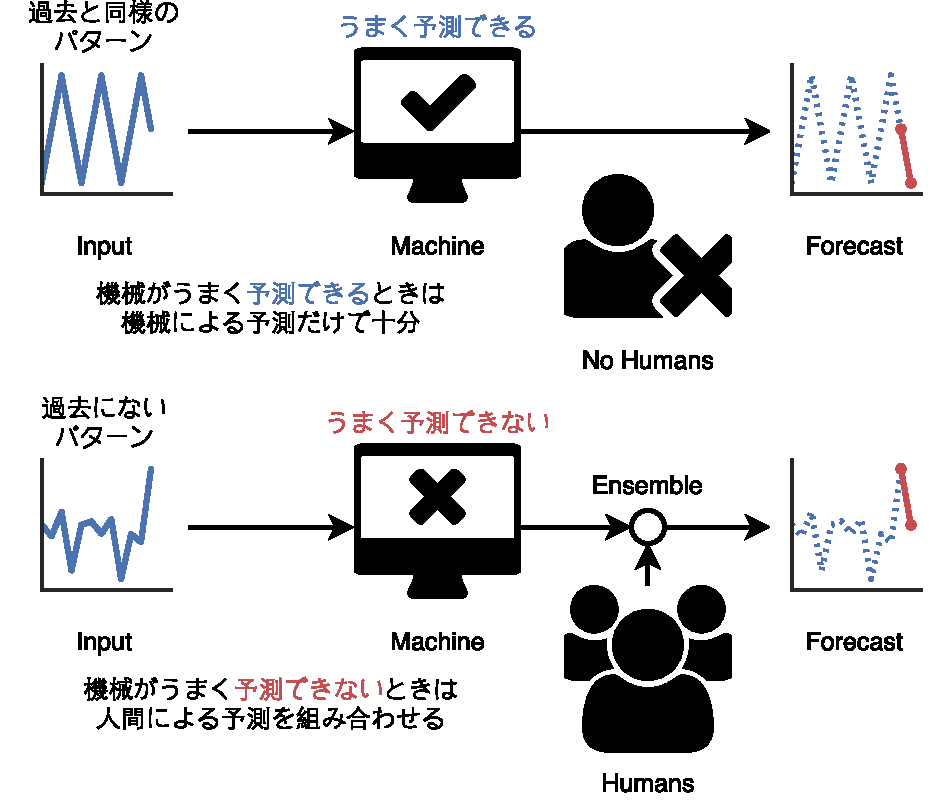
\includegraphics[width=\textwidth]{slide-schematic.pdf}
          \caption{従来手法の問題に対する本研究のアプローチ}
        \end{figure}
      \end{column}
    \end{columns}
  \end{block}
  %%%%%%%%%%%%%%%%%%%%%%%%%%%%%%%%%%%%%%%%%%%%%%%%%%%%%%%%%%%%%%%%

  %%%%%%%%%%%%%%%%%%%%%%%%%%%%%%%%%%%%%%%%%%%%%%%%%%%%%%%%%%%%%%%%
  \begin{block}{提案手法: 人間と機械のアンサンブル法}
    \begin{columns}
      \begin{column}{.44\textwidth}
        \begin{itembox}[l]{\structure{入力に応じた誤差の期待値を表現するモデル}}
          予測器$\theta$は,\alert{入力$\x$に対する事後分布$f_\theta(y|\x)$を出力}する
          \begin{itemize}
            \item 分布の平均を予測値$y_\theta(\x)$とする
            \item 分布の\alert{分散$\varm$を二乗誤差の期待値とみなす}
          \end{itemize}
          \begin{figure}
            \centering
            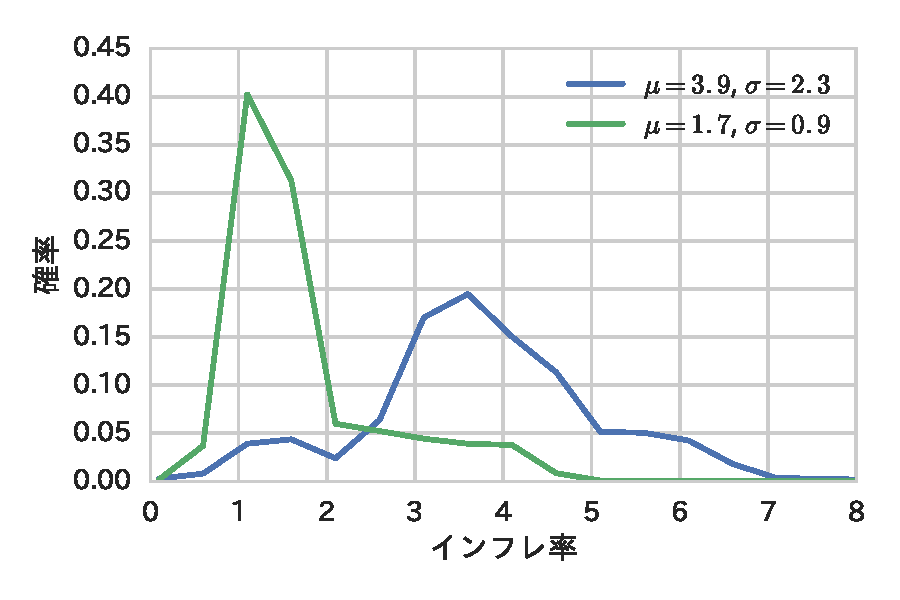
\includegraphics[width=.9\textwidth]{poster-machine_outputs.pdf}
            \caption{予測器が出力した分布の例.青より緑の方が分散$=$誤差の期待値が小さい}
          \end{figure}
        \end{itembox}
        \hfill
      \end{column}
      %%%%%%%%%%%%%%%%%%%%%%%%%%%%%%%%%%%%%%%%%%%%%%%%%%%%%%%%%%%%%%%%
      \begin{column}{.54\textwidth}
        \begin{itembox}[l]{\structure{誤差の期待値を最小化する人間と機械の組み合わせ}}
          $n$人の人間$h_1,\dots,h_n$と1つの機械$\theta$の予測の平均をアンサンブルの予測$Y_{\theta,h}(n|\x)$とし,その\alert{二乗誤差の期待値$\MSE[Y_{\theta,h}(n|\x)]$を最小化する人数$n^\ast$を求める}
          \begin{equation*}
            \MSE[Y_{\theta,h}(n|\x)]
              = \frac{n\varh + \varm + n(n - 1)\covh + 2n\covmh}{{(n + 1)}^2}
            \label{eq: expected squared error}
          \end{equation*}
          \begin{figure}
            \centering
            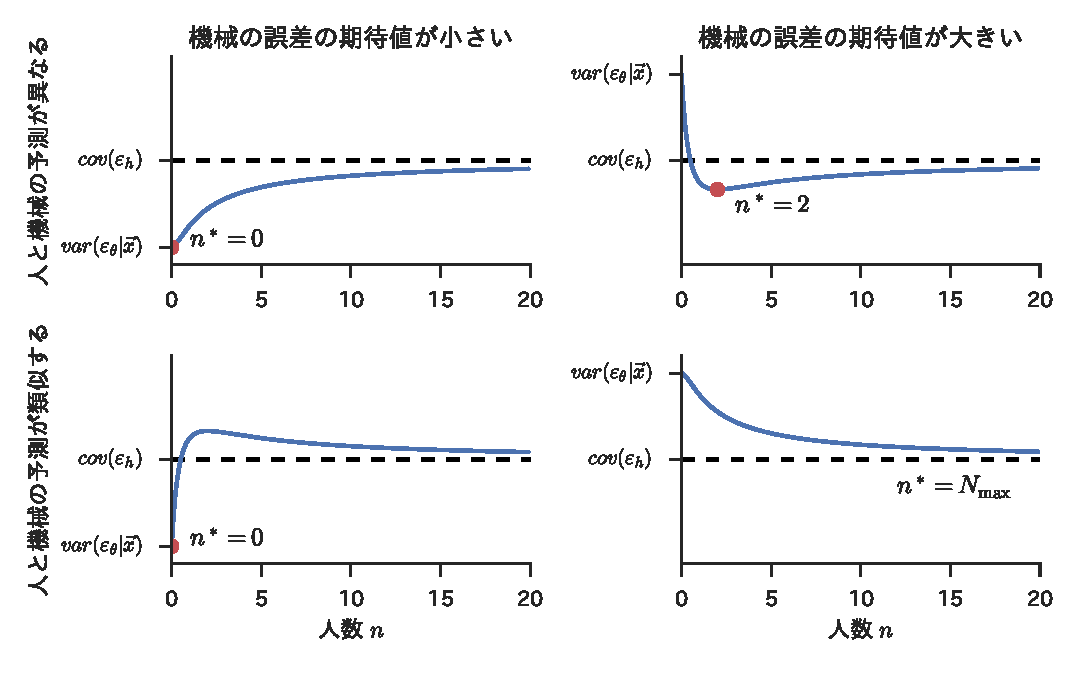
\includegraphics[width=.8\textwidth]{poster-ensemble_graph.pdf}
            \caption{人数$n$に関するアンサンブルの二乗誤差の期待値$\MSE[Y_{\theta,h}(n|\x)]$のグラフ}
          \end{figure}
        \end{itembox}
      \end{column}
    \end{columns}
  \end{block}
  %%%%%%%%%%%%%%%%%%%%%%%%%%%%%%%%%%%%%%%%%%%%%%%%%%%%%%%%%%%%%%%%

  %%%%%%%%%%%%%%%%%%%%%%%%%%%%%%%%%%%%%%%%%%%%%%%%%%%%%%%%%%%%%%%%
  \begin{block}{実験: アメリカのインフレ予測への適用}
    \begin{columns}
      \begin{column}{.49\textwidth}
        \structure{予測対象}
        \begin{itemize}
          \item アメリカのインフレに関する4つの指標の年間変化率
          \item CPI,Core CPI,PCE,Core PCE (1959--2016)
        \end{itemize}
        \smallskip
        \structure{予測手法}
        \begin{itemize}
          \item ベンチマーク: 自己回帰移動平均モデル ARMA(1,1)
          \item 機械: 再帰型ニューラルネット (RNN)
          \item 人間: 経済予測の調査データ Livingston Survey (LIV) と SPF
          \item 提案手法: 機械 (RNN) と人間 (LIV, SPF) の組み合わせにより構成
        \end{itemize}
        \smallskip
        \structure{評価方法}
        \begin{itemize}
          \item 2008年以前を訓練セット,それ以降をテストセットに分割
          \item 予測精度の評価指標に二乗平均平方根誤差 (RMSE) を使用
        \end{itemize}
        \smallskip
        \begin{table}
          \caption{ベンチマークを1とした相対 RMSE}
          \begin{center}
            % \small
            \begin{tabular}{lrrrrrrr}
\toprule
{} &  CPI-LIV &  CPI-SPF &  CoreCPI &    PCE &  CorePCE &  CPI-6M &  CPI-1998 \\
\midrule
ベンチマーク&    1.000 &    1.000 &    1.000 &  1.000 &    1.000 &   1.000 &     1.000 \\
機械      &    0.889 &    0.889 &    0.788 &  0.933 &    0.842 &   1.010 &     0.941 \\
人間      &    0.704 &\alert{0.736}&\alert{0.767}&\alert{0.711}&    0.848 &   0.939 &     0.940 \\
提案手法   &\alert{0.689}&\alert{0.736}&\alert{0.767}&  0.724 &\alert{0.827}&\alert{0.931} &\alert{0.755} \\
\bottomrule
\end{tabular}

          \end{center}
        \end{table}
        \begin{itembox}[l]{\structure{結果1}}
          \alert{提案手法は7つのうち4つで最も精度が高く,2つで既存手法と同じになった}
        \end{itembox}
      \end{column}
      %%%%%%%%%%%%%%%%%%%%%%%%%%%%%%%%%%%%%%%%%%%%%%%%%%%%%%%%%%%%%%%%
      \begin{column}{.49\textwidth}
        \begin{figure}
          \centering
          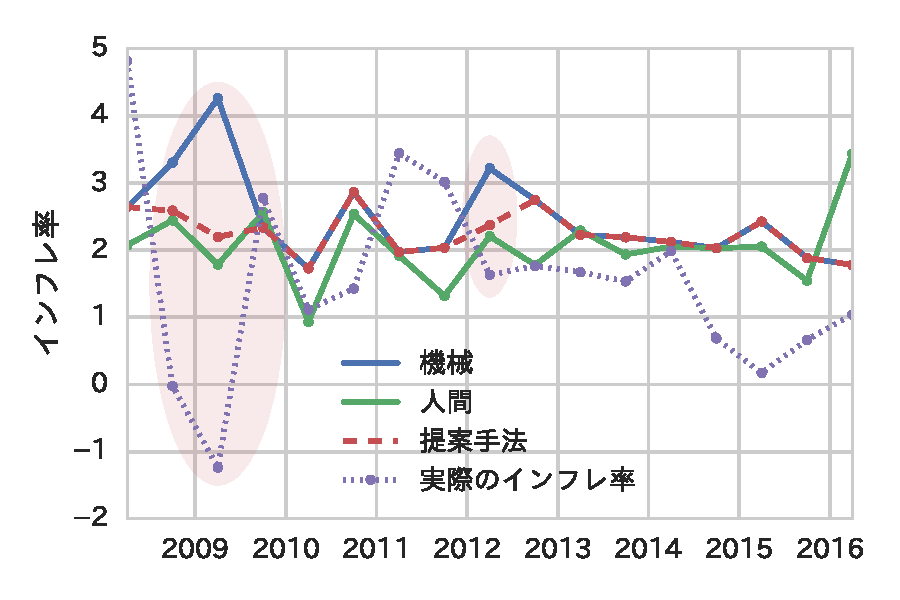
\includegraphics[width=.85\columnwidth]{poster-behavior.pdf}
          \caption{テストセットにおける各手法の予測}
          \centering
        \end{figure}
        \begin{itembox}[l]{\structure{結果2}}
          \alert{2008年9月のリーマンショック後,提案手法は機械の誤差が大きいとき人間による予測を利用することで誤差を小さくした}
        \end{itembox}
      \end{column}
    \end{columns}
  \end{block}
  %%%%%%%%%%%%%%%%%%%%%%%%%%%%%%%%%%%%%%%%%%%%%%%%%%%%%%%%%%%%%%%%
  % \scriptsize
  % \bibliographystyle{plain}
  % \bibliography{../paper/master-thesis}
\end{frame}
\end{document}
